\section{Campo magnético: condutor retilíneo}

\frame{
	\frametitle{O campo magnético gerado por correntes elétricas}
	\begin{block}{História}
		Estudou-se, por muito tempo, as propriedades dos ímãs sem estabelecer qualquer relação com os \textbf{fenômenos elétricos}.
		\begin{itemize}
			\item Em 1820, acidentalmente, segundo algumas versões, em uma de suas aulas, um professor de Amsterdã deixou uma pequena \textbf{bússola sob um circuito elétrico} e verificou que sua agulha era defletida quando se ligava o circuito. Esse professor, Hans Christian Oersted, repetiu várias vezes a experiência, concluindo que \textbf{toda corrente elétrica gera ao redor de si um campo magnético}.
		\end{itemize}
	\end{block}
}

\frame{
	\frametitle{O campo magnético gerado por correntes elétricas}
	\centerline{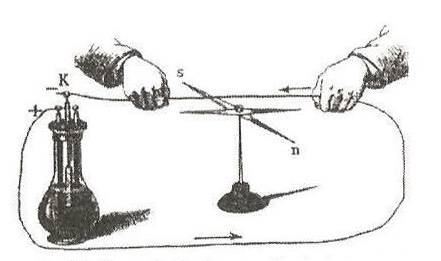
\includegraphics[width=0.9\linewidth]{Figuras/Ch07/fig1.jpg}}
}

\frame{
	\frametitle{O campo magnético gerado por correntes elétricas}
	\begin{block}{Mas e agora?}
		Oersted concluiu que, a exemplo dos ímãs, toda corrente elétrica gera, no espaço ao seu redor, um campo magnético.
		\begin{itemize}
			\item A grande pergunta é: \textbf{qual a direção e o sentido de desvio dessa agulha?} Geralmente encontramos dificuldades para determinar a direção e o sentido do vetor indução $\vec{B}$. A forma mais fácil para se determinar essa direção e sentido é a utilização da \textbf{regra da mão direita}.
		\end{itemize}
	\end{block}
}

\frame{
	\frametitle{Regra da mão direita}
	\begin{block}{Importância}
		É uma regra muito útil para se determinar o \textbf{sentido do vetor indução magnética $\vec{B}$} num ponto do campo gerado por uma corrente elétrica.
		\begin{itemize}
			\item O \textbf{polegar da mão direita} indica o \textbf{sentido da corrente elétrica} que está atravessando o fio.
			\item Os \textbf{demais dedos semidobrados} envolvem o condutor e fornecem o sentido de $\vec{B}$ num ponto $P$.
		\end{itemize}
	\end{block}
}

\frame{
	\frametitle{Regra da mão direita}
	\begin{block}{Nomenclatura}
		O vetor indução magnética $\vec{B}$ é \textbf{perpendicular} a $P$.
		\begin{itemize}
			\item Em direções perpendiculares à uma folha de papel, por exemplo, é comum utilizarmos os termos \textbf{saindo do plano} e \textbf{entrando no plano}, para facilitar a representação dos vetores.
		\end{itemize}
	\end{block}

	\vspace{0.3cm}
	
	\centering
	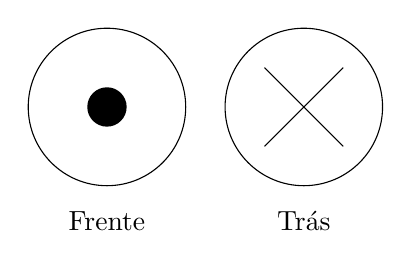
\begin{tikzpicture}[x=1cm,y=1cm]
		\draw (0,0) circle (1) node[below=1.2cm] {Frente} (2.5,0) circle (1) node[below=1.2cm] {Trás} (2.5,0) -- ++(0.5,0.5) -- ++(-1,-1) ++(0,1) -- ++(1,-1);
		\fill (0,0) circle (0.25);
	\end{tikzpicture}
%	\centerline{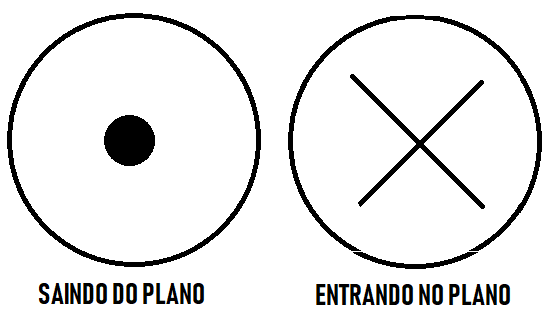
\includegraphics[width=0.4\linewidth]{Figuras/Ch07/fig3.png}}
}

\frame{
	\frametitle{Regra da mão direita - Exemplos}
	\centerline{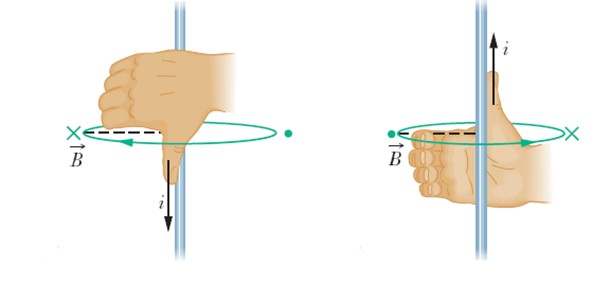
\includegraphics[width=0.7\linewidth]{Figuras/Ch07/fig4.jpg}}
	\vspace{0.2cm}
	\centerline{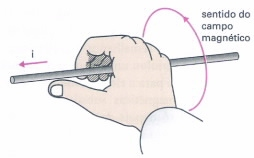
\includegraphics[width=0.5\linewidth]{Figuras/Ch07/fig5.jpg}}
}

\frame{
	\frametitle{Campo magnético num condutor retilíneo}
	\begin{block}{Definição}
		Um \textbf{fio retilíneo e muito longo} é percorrido por corrente elétrica e, em seu entorno, estabelece-se um campo magnético. Seja $P$ um ponto do campo. O vetor indução magnética $\vec{B}$ em $P$ tem as seguintes características:
		\begin{itemize}
			\item \textbf{Direção}: perpendicular ao plano e definido pelo fio e pelo ponto $P$.
			\item \textbf{Sentido}: dada pela regra da mão direita.
			\item \textbf{Intensidade}: dada pela Lei de Biot-Savart.
		\end{itemize}
	\end{block}
}

\frame{
	\frametitle{Lei de Biot-Savart}
	\begin{block}{Definição}
		A intensidade de $\vec{B}$ ($ |\vec{B}| $) depende da intensidade da corrente $i$, da distância $d$ entre o ponto $P$ e o fio, e do meio onde o fio se encontra.
		\begin{itemize}
			\item A grandeza que leva em conta o meio é $\mu$ (permeabilidade magnética do meio). Para o vácuo $\mu = \SI{4\pi e-7}{\tesla\meter\per\ampere}$.
		\end{itemize}
		\vspace{0.3cm}
		$$\boxed{|\vec{B}| = \dfrac{\mu \cdot i}{2\pi \cdot d}}$$
		\begin{itemize}
			\item A unidade de campo magnético no SI é \textbf{Tesla} (\si{\tesla}).
		\end{itemize}
	\end{block}
}

\frame{
	\frametitle{Campo magnético num condutor retilíneo - Exemplo $\#01$}
	\begin{block}{}
		Suponha que temos um fio percorrido por uma corrente de intensidade igual a \SI{5}{\ampere}. Determine o campo magnético de um ponto situado a \SI{2}{\centi\meter} do fio.
	\end{block}

	\vspace{0.2cm}
	\begin{block}{Resolução}
		$$|\vec{B}| = \dfrac{\mu \cdot i}{2\pi \cdot d} = \dfrac{\num{4\pi e-7} \cdot 5}{2\pi \cdot \num{0,02}} = \SI{5e-5}{\tesla}$$
	\end{block}
}

\frame{
	\frametitle{Campo magnético num condutor retilíneo - Exemplo $\#02$}
	\begin{block}{}
		Imagine dois fios retos e longos, percorridos pelas correntes elétricas $i_1 = \SI{3}{\ampere}$ e $i_2 = \SI{4}{\ampere}$. Os sentidos de tráfego das correntes em ambos os fios são de baixo para cima. Considerando o vácuo como o meio, determine o módulo, a direção e o sentido do campo magnético resultante em um ponto $P$, distante de \SI{2}{\centi\meter} do fio 1 e \SI{4}{\centi\meter} do fio 2.
	\end{block}
	
	\vspace{0.2cm}
	\begin{block}{Resolução}
		\begin{itemize}
			\item $|\vec{B_1}| = \dfrac{\mu \cdot i}{2\pi \cdot d} = \dfrac{\num{4\pi e-7} \cdot 3}{2\pi \cdot \num{0,02}} = \SI{3e-5}{\tesla}$ (entrando no plano). \\
			      \vspace{0.2cm}
			\item $|\vec{B_2}| = \dfrac{\mu \cdot i}{2\pi \cdot d} = \dfrac{\num{4\pi e-7} \cdot 4}{2\pi \cdot \num{0,04}} = \SI{2e-5}{\tesla}$ (saindo do plano). \\
			      \vspace{0.2cm}
			\item $|\vec{B_R}| = |\vec{B_1}| - |\vec{B_2}| = \SI{1e-5}{\tesla}$ (entrando no plano).
		\end{itemize}
	\end{block}
}

\section*{Exercícios}
\frame{
	\frametitle{Exercícios}
	\begin{block}{}
		01. Um topógrafo está usando uma bússola a \SI{6}{\meter} abaixo de uma linha de transmissão na qual existe uma corrente constante de \SI{100}{\ampere}. Qual é o valor do campo magnético no local da bússola em virtude da linha de transmissão?
		\vspace{0.4cm}

		02. Dois fios retilíneos, longos e paralelos, são atravessados por correntes elétricas de intensidades iguais, respectivamente, a \SI{1}{\ampere} e \SI{2}{\ampere}. Os sentidos de tráfego das correntes são opostos e os fios estão distanciados \SI{2}{\meter}. Determine a intensidade do vetor campo magnético num ponto equidistante dos fios, no plano formado por eles.
		\vspace{0.4cm}

		03. (UNESP-SP) Um fio longo e retilíneo é percorrido por uma corrente elétrica constante $i$ e o vetor indução magnética em um ponto próximo ao fio tem intensidade $\vec{B}$. Se o mesmo fio for percorrido por uma corrente elétrica constante igual a $3i$, determine a intensidade do vetor indução magnética no mesmo ponto próximo ao fio.
	\end{block}
}

\section*{Referências}
\frame{
	\frametitle{Referências e Exercícios Complementares}
	\begin{itemize}
		\item ALEXANDRE, Charles K.; SADIKU, Matthew N. O. Fundamentos de Circuitos Elétricos. 5. ed. Porto Alegre: AMGH, 2013.
	\end{itemize}
	%\centering{\alert{Página 36 - \textbf{1.6.1 até 1.6.5, 1.6.17 até 1.6.19}}} \\
	\centering{\alert{Lista de exercícios 07}}
}
